% Options for packages loaded elsewhere
% Options for packages loaded elsewhere
\PassOptionsToPackage{unicode}{hyperref}
\PassOptionsToPackage{hyphens}{url}
\PassOptionsToPackage{dvipsnames,svgnames,x11names}{xcolor}
%
\documentclass[
  letterpaper,
  DIV=11,
  numbers=noendperiod]{scrreprt}
\usepackage{xcolor}
\usepackage{amsmath,amssymb}
\setcounter{secnumdepth}{5}
\usepackage{iftex}
\ifPDFTeX
  \usepackage[T1]{fontenc}
  \usepackage[utf8]{inputenc}
  \usepackage{textcomp} % provide euro and other symbols
\else % if luatex or xetex
  \usepackage{unicode-math} % this also loads fontspec
  \defaultfontfeatures{Scale=MatchLowercase}
  \defaultfontfeatures[\rmfamily]{Ligatures=TeX,Scale=1}
\fi
\usepackage{lmodern}
\ifPDFTeX\else
  % xetex/luatex font selection
\fi
% Use upquote if available, for straight quotes in verbatim environments
\IfFileExists{upquote.sty}{\usepackage{upquote}}{}
\IfFileExists{microtype.sty}{% use microtype if available
  \usepackage[]{microtype}
  \UseMicrotypeSet[protrusion]{basicmath} % disable protrusion for tt fonts
}{}
\makeatletter
\@ifundefined{KOMAClassName}{% if non-KOMA class
  \IfFileExists{parskip.sty}{%
    \usepackage{parskip}
  }{% else
    \setlength{\parindent}{0pt}
    \setlength{\parskip}{6pt plus 2pt minus 1pt}}
}{% if KOMA class
  \KOMAoptions{parskip=half}}
\makeatother
% Make \paragraph and \subparagraph free-standing
\makeatletter
\ifx\paragraph\undefined\else
  \let\oldparagraph\paragraph
  \renewcommand{\paragraph}{
    \@ifstar
      \xxxParagraphStar
      \xxxParagraphNoStar
  }
  \newcommand{\xxxParagraphStar}[1]{\oldparagraph*{#1}\mbox{}}
  \newcommand{\xxxParagraphNoStar}[1]{\oldparagraph{#1}\mbox{}}
\fi
\ifx\subparagraph\undefined\else
  \let\oldsubparagraph\subparagraph
  \renewcommand{\subparagraph}{
    \@ifstar
      \xxxSubParagraphStar
      \xxxSubParagraphNoStar
  }
  \newcommand{\xxxSubParagraphStar}[1]{\oldsubparagraph*{#1}\mbox{}}
  \newcommand{\xxxSubParagraphNoStar}[1]{\oldsubparagraph{#1}\mbox{}}
\fi
\makeatother


\usepackage{longtable,booktabs,array}
\usepackage{calc} % for calculating minipage widths
% Correct order of tables after \paragraph or \subparagraph
\usepackage{etoolbox}
\makeatletter
\patchcmd\longtable{\par}{\if@noskipsec\mbox{}\fi\par}{}{}
\makeatother
% Allow footnotes in longtable head/foot
\IfFileExists{footnotehyper.sty}{\usepackage{footnotehyper}}{\usepackage{footnote}}
\makesavenoteenv{longtable}
\usepackage{graphicx}
\makeatletter
\newsavebox\pandoc@box
\newcommand*\pandocbounded[1]{% scales image to fit in text height/width
  \sbox\pandoc@box{#1}%
  \Gscale@div\@tempa{\textheight}{\dimexpr\ht\pandoc@box+\dp\pandoc@box\relax}%
  \Gscale@div\@tempb{\linewidth}{\wd\pandoc@box}%
  \ifdim\@tempb\p@<\@tempa\p@\let\@tempa\@tempb\fi% select the smaller of both
  \ifdim\@tempa\p@<\p@\scalebox{\@tempa}{\usebox\pandoc@box}%
  \else\usebox{\pandoc@box}%
  \fi%
}
% Set default figure placement to htbp
\def\fps@figure{htbp}
\makeatother





\setlength{\emergencystretch}{3em} % prevent overfull lines

\providecommand{\tightlist}{%
  \setlength{\itemsep}{0pt}\setlength{\parskip}{0pt}}



 


\KOMAoption{captions}{tableheading}
\makeatletter
\@ifpackageloaded{bookmark}{}{\usepackage{bookmark}}
\makeatother
\makeatletter
\@ifpackageloaded{caption}{}{\usepackage{caption}}
\AtBeginDocument{%
\ifdefined\contentsname
  \renewcommand*\contentsname{Table of contents}
\else
  \newcommand\contentsname{Table of contents}
\fi
\ifdefined\listfigurename
  \renewcommand*\listfigurename{List of Figures}
\else
  \newcommand\listfigurename{List of Figures}
\fi
\ifdefined\listtablename
  \renewcommand*\listtablename{List of Tables}
\else
  \newcommand\listtablename{List of Tables}
\fi
\ifdefined\figurename
  \renewcommand*\figurename{Figure}
\else
  \newcommand\figurename{Figure}
\fi
\ifdefined\tablename
  \renewcommand*\tablename{Table}
\else
  \newcommand\tablename{Table}
\fi
}
\@ifpackageloaded{float}{}{\usepackage{float}}
\floatstyle{ruled}
\@ifundefined{c@chapter}{\newfloat{codelisting}{h}{lop}}{\newfloat{codelisting}{h}{lop}[chapter]}
\floatname{codelisting}{Listing}
\newcommand*\listoflistings{\listof{codelisting}{List of Listings}}
\makeatother
\makeatletter
\makeatother
\makeatletter
\@ifpackageloaded{caption}{}{\usepackage{caption}}
\@ifpackageloaded{subcaption}{}{\usepackage{subcaption}}
\makeatother
\usepackage{bookmark}
\IfFileExists{xurl.sty}{\usepackage{xurl}}{} % add URL line breaks if available
\urlstyle{same}
\hypersetup{
  pdftitle={Rachel Elnora Mannuelle Sidanta},
  pdfauthor={18224125 Rachel Elnora Mannuelle Sidanta},
  colorlinks=true,
  linkcolor={blue},
  filecolor={Maroon},
  citecolor={Blue},
  urlcolor={Blue},
  pdfcreator={LaTeX via pandoc}}


\title{Rachel Elnora Mannuelle Sidanta}
\usepackage{etoolbox}
\makeatletter
\providecommand{\subtitle}[1]{% add subtitle to \maketitle
  \apptocmd{\@title}{\par {\large #1 \par}}{}{}
}
\makeatother
\subtitle{Portfolio Asesmen II-2100 KIPP}
\author{18224125 Rachel Elnora Mannuelle Sidanta}
\date{2027-06-10}
\begin{document}
\maketitle

\renewcommand*\contentsname{Table of contents}
{
\hypersetup{linkcolor=}
\setcounter{tocdepth}{2}
\tableofcontents
}

\bookmarksetup{startatroot}

\chapter*{Selamat Berjumpa}\label{selamat-berjumpa}
\addcontentsline{toc}{chapter}{Selamat Berjumpa}

\markboth{Selamat Berjumpa}{Selamat Berjumpa}

\begin{figure}[H]

{\centering \includegraphics[width=9.5\linewidth,height=\textheight,keepaspectratio]{images/AZRL.png}

}

\caption{About Me}

\end{figure}%

Armein Z R Langi adalah Guru Besar di Sekolah Teknik Elektro dan
Informatika ITB, dosen ITB sejak Desember 1987, mantan Rektor
Universitas Kristen Maranatha, 1 Maret 2016 s/d 29 Februari 2020, mantan
Kepala Pusat Penelitian Teknologi Informasi dan Komunikasi (PP-TIK) ITB
November 2005 s/d Maret 2010, dan Sekretaris MWA ITB Mei 2010-Jan 2011.

Lahir di Tomohon 1962 dari pasangan Manado dan Sunda. Saat ini tinggal
di Bandung, menikah dengan Ina dan dikaruniai empat anak. Ayah dari
Gladys, Kezia, Andria, dan Marco.

Sharing pikiran singkat ada di blog \url{https://azrl.wordpress.com}.
Facebookk: armein\_langi

Andria, putri saya, lumayan sering membaca blog ini. Dia juga sumber
inspirasi tulisan saya. Dia senang menceritakan jokes pada saya, dan
kalau bagus saya tulis di sini, terutama seri Kocak Ala Andria. Dan dia
suka heran, karena isinya sudah berbeda. Memang saya senang
mengubah-ngubah cerita karena saya tidak suka menjiplak mentah-mentah.
Minggu lalu tidak sengaja dia memuji tulisan blog ini.

``Papa\ldots{} papa\ldots{} ``, tanyanya, ``Tulisan blog papa itu
copy-paste dari tulisan orang ya\ldots?''

Haa? Ya nggak mungkin lah. Kecuali lirik lagu, semua artikel di sini
ditulis sendiri.

``Ah bohong, soalnya tulisannya terlalu banyak\ldots.'' katanya tetap
tidak percaya, ``Nggak mungkinlah papa tulis sendiri\ldots{}''

Hehe, saya tersenyum sambil membelai Andria, karena buat saya itu adalah
ultimate compliment. Thanks sweetheart\ldots{}

Jadi kalau orang tidak percaya bahwa sesuatu itu karya anda, anda yang
buat, jangan marah. Itu adalah pujian yang sejati.

\bookmarksetup{startatroot}

\chapter{UTS-1 All About Me （╹◡╹）}\label{uts-1-all-about-me}

\begin{figure}[H]

{\centering \includegraphics[width=9.5\linewidth,height=\textheight,keepaspectratio]{All_About_me/../images/IMG_3738.JPEG}

}

\caption{About Me}

\end{figure}%

\section{\texorpdfstring{\textbf{About Me
(｡•̀ᴗ-)✧}}{About Me (｡•̀ᴗ-)✧}}\label{about-me-ux1d17-}

Aku Rachel Elnora Mannuelle Sidanta, mahasiswa Sistem dan Teknologi
Informasi angkatan 2024 di STEI-K ITB. Aku berasal dari Semarang, Jawa
Tengah (\#jawir) dan dulu menempuh pendidikan di SMA Kolese Loyola. Saat
ini, aku tinggal di Jatinangor, yah Bandung geser sedikit lah kalau bisa
dibilang.

Hidup jauh dari rumah bukan masalah besar bagiku, karena aku tidak
sendirian. Aku punya Ahmad Zaky Robbani yang baik hati, tidak sombong,
murah hati, murah senyum, pantang menyerah, berjiwa ksatria, dermawan,
ganteng, tinggi, feminis, 6'4'' (ini klaim sepihak sih), cat enthusiast,
dan mie ayam lover.

\section{\texorpdfstring{\textbf{Hobi dan Minat
(⁄⁄\textgreater⁄▿⁄\textless⁄⁄)♡}}{Hobi dan Minat (⁄⁄\textgreater⁄▿⁄\textless⁄⁄)♡}}\label{hobi-dan-minat}

Kalau lagi introvert, aku suka mendengarkan lagu-lagu di playlist
Spotify-ku, main gitar tipis-tipis, atau sekadar scroll IG, TikTok, dan
X. Tapi kalau lagi ekstrovert, aku suka main kartu, board game, atau
billiard. Pokoknya apa aja aku ayo.

Aku suka alam --- naik gunung atau trekking tipis kalau lagi nggak ada
waktu. Di luar itu, aku suka explore hal-hal random di internet, hal
yang memang sejalan dengan jurusanku.

Selain itu, ini kebiasaan dari dulu, aku suka jadi orang (sok) sibuk
karena sekali manit bisa 3-5 sekaligus.

\section{\texorpdfstring{\textbf{Nilai yang Aku Pegang (´• ω
•`)ﾉ}}{Nilai yang Aku Pegang (´• ω •`)ﾉ}}\label{nilai-yang-aku-pegang-ux3c9-uxff89}

Beberapa waktu lalu aku nemu kalimat dari akun X @unniemara: \emph{``You
never really know what someone's going through. Be kind. Always. Even
when they don't look like they need it.''}

Kalimat itu nempel banget di kepalaku. Aku belajar buat nggak gampang
menilai orang dari luar, dan berusaha jadi orang baik bagi siapapun di
sekitarku. Dunia udah cukup berat, jadi aku mau menjadi seseorang yang
bisa bikin orang lain ngerasa lebih tenang.

\section{\texorpdfstring{\textbf{Gagasan yang Sedang Aku Pikirkan
(⌒▽⌒)☆}}{Gagasan yang Sedang Aku Pikirkan (⌒▽⌒)☆}}\label{gagasan-yang-sedang-aku-pikirkan}

Semester lalu, aku merasa belum cukup memahami bidang informatika. Itu
jadi komitmen pertamaku ketika dilantik sebagai anggota biasa HMIF ITB:
menyelami berbagai jalur karier di dunia informatika untuk menemukan
bidang yang paling sesuai dengan minat dan potensiku. Sekarang aku
memiliki kesempatan emas di Inkubator IT (IIT) HMIF ITB, divisi Media
Intelligence. Di situ kami akan menerima client nyata, dan aku bisa
belajar melalui project-project secara langsung.

\section{\texorpdfstring{\textbf{Kesimpulan: Kisahku Masih dalam Draft
Pertama ( ˘͈ ᵕ
˘͈♡)}}{Kesimpulan: Kisahku Masih dalam Draft Pertama ( ˘͈ ᵕ ˘͈♡)}}\label{kesimpulan-kisahku-masih-dalam-draft-pertama-ux1d55}

Pada akhirnya, aku sadar kalau aku nggak perlu menunggu untuk menjadi
``seseorang yang sudah jadi'' untuk mulai bercerita. Proses pencarian
jati diri ini sendiri adalah cerita yang menarik untuk ditulis.
Tujuannya bukan menjadi protagonis yang sempurna tanpa konflik, tapi
menjadi penulis yang berani mengubah halaman-halaman buruk menjadi bab
pembuka untuk pertumbuhan.

Kisahku masih berjalan, dan aku --- dengan segala kekurangan dan
kebingunganku --- adalah satu-satunya orang yang berhak memegang pena
itu.

\bookmarksetup{startatroot}

\chapter{UTS-2 My Songs for You
♫（´▽｀）♪}\label{uts-2-my-songs-for-you}

Belakangan ini aku lagi suka banget sama Oasis. Salah satu lagu
favoritku adalah Don't Go Away. Setiap kali kudengar, lagu itu seperti
mengulang kembali semua rasa yang kutemukan pada seseorang yang sangat
aku cintai dan selalu ada di sisiku.

Lagu itu bercerita tentang takut kehilangan, tentang seseorang yang
ingin waktu berhenti sejenak agar orang yang dicintainya tak pergi.
Tentang hal-hal sederhana yang justru paling sulit diungkapkan:
``tetaplah di sini, cukup itu saja.''

Dari situ, aku terinspirasi untuk menulis lagu yang punya makna serupa.
Sebuah cara kecil untuk menyimpan perasaan yang tak selalu bisa
disampaikan dengan kata-kata.

p.s. lagu ini pernah aku selipkan di surat pertamaku untuknya.

\section{\texorpdfstring{\textbf{Stay a Little
While}}{Stay a Little While}}\label{stay-a-little-while}

\emph{Inspired by ``Don't Go Away'' by Oasis}

Lyrics and composition by Rachel Elnora

Key: C Major

{[}Verse 1{]}

Cold night turns to morning, the sky's a shade of grey

And your name caught in my mind

While the world keeps turning, I watch it fade away

Things I meant got left behind

{[}Pre-Chorus{]}

I don't wanna lose you when the lights go down

I don't wanna watch you when you're not around

{[}Chorus{]}

So stay a little while, say what you feel

Say that you'll stay for more than a while

You're part of my days, 'cause I need more time

Yes, I need more time just to make you smile

{[}Verse 2{]}

Blame my hesitation, the words I couldn't say

All dreams we've left inside

Blame the constellations, they took your gaze away

Left my heart a step behind

{[}Pre-Chorus{]}

I still wanna find you when the rain falls down

I still wanna hold you when there's no sound

{[}Chorus{]}

So stay a little while, say what you feel

Say that you'll stay for more than a while

You're part of my days, 'cause I need more time

Yes, I need more time just to make you smile

{[}Bridge{]}

Me and you, what's going on?

Maybe love's just learning to be strong

{[}Chorus{]} (Reprise)

So stay a little while, say what you feel

Say that you'll stay for more than a while

You're part of my days, 'cause I need more time

Yes, I need more time just to make you smile

Yes, I need more time just to make you smile

Yes, I need more time just to make you smile

So stay a little while

\bookmarksetup{startatroot}

\chapter{UTS-3 My Stories for You
(๑˘︶˘๑)}\label{uts-3-my-stories-for-you-uxe51uxe51}

Semester pertama di ITB bukan masa yang mudah untukku. Aku datang dengan
semangat tinggi, tapi kenyataan menampar cukup keras. IP-ku semester 1
hanya sekitar 2,7. Rasanya berat sekali, apalagi itu masih masa TPB,
saat semua orang bilang mata kuliahnya masih ``se-level SMA''. Aku
sempat kehilangan arah dan percaya diri.

Waktu itu aku juga sempat sedih ketika hasil peminatan keluar dan aku
ditempatkan di Sistem dan Teknologi Informasi - Jatinangor. Aku memang
mendapat jurusan yang kuinginkan, tapi bukan di kampus yang kuimpikan.
Semua terasa tidak sesuai harapan. Aku mulai mempertanyakan banyak hal
--- tentang kemampuan, pilihan, bahkan diriku sendiri.

Lalu aku bertemu seseorang. Awalnya kami hanya teman. Kami sering
berangkat bareng, makan dan main bareng, kadang belajar bareng. Aku dulu
tipe yang harus belajar sendiri karena merasa hanya bisa paham kalau
berjuang sendirian. Tapi suatu hari, aku benar-benar tidak bisa mengerti
padahal esoknya adalah hari praktikum, dan dia dengan sabar
mengajarkannya padaku. Saat itu, aku sadar aku jatuh cinta.

Sekarang dia adalah pacarku. Kami beda jurusan --- dia di IF, aku di STI
--- tapi itu tidak membuat kami jauh. Kami tetap belajar bersama, saling
mendukung, dan saling mengisi kekurangan satu sama lain. Saat aku mulai
ragu pada diri sendiri, dia selalu memberi semangat dan meyakinkanku.

Semester 2, IP-ku naik jadi 3,5. Dan lebih dari angka itu, aku belajar
bahwa keberhasilan tidak selalu soal kerja keras sendirian, tapi juga
tentang siapa yang ada di sisimu waktu kamu hampir menyerah.

\bookmarksetup{startatroot}

\chapter{UTS-4 My SHAPE (Spiritual Gifts, Heart, Abilities, Personality,
Experiences)
(✿˘▽˘)っ}\label{uts-4-my-shape-spiritual-gifts-heart-abilities-personality-experiences-ux3063}

\begin{quote}
\textbf{Tujuan:} Merangkum rancangan diri (charter) agar aku melayani,
berkarya, dan memimpin secara paling selaras dengan karunia dan
pengalaman hidupku. Dapat langsung ditempel ke halaman \textbf{UTS-4 ---
My SHAPE} dan dipakai sebagai acuan aksi 90 hari.
\end{quote}

\section{0) Ringkasan 1 Halaman}\label{ringkasan-1-halaman}

\textbf{Peran Inti:} Komunikator kreatif dan penggerak komunitas yang
menggabungkan seni, teknologi, dan nilai kemanusiaan.

\textbf{Misi:} Membagikan pesan positif dan menggerakkan orang lewat
karya visual, tulisan, dan teknologi yang bermakna.

\textbf{Kekuatan Utama:} Menulis dan merancang konten, berpikir
sistematis, bekerja dalam tim, dan menjaga suasana positif.

\textbf{Dampak yang Dituju:} Menciptakan ruang belajar, karya, dan
komunitas yang membuat orang merasa terhubung, dipahami, dan bersemangat
berkembang.

\textbf{Peta SHAPE (singkat):}

\begin{itemize}
\tightlist
\item
  \textbf{S --- Spiritual Gifts:} Encouragement, Creativity, Leadership,
  Empathy, Communication.
\item
  \textbf{H --- Heart (Minat \& Cinta Pelayanan):} Media kreatif,
  pelayanan sosial, lingkungan hidup, pendidikan, dan relasi antar
  manusia.
\item
  \textbf{A --- Abilities (Kemampuan):} Desain visual, penulisan
  kreatif, komunikasi publik, dokumentasi, koordinasi acara, dan
  teknologi.
\item
  \textbf{P --- Personality (Gaya Kepribadian Kerja):} Reflektif,
  kolaboratif, dan terencana.
\item
  \textbf{E --- Experiences (Pengalaman Kunci):} Organisasi sekolah dan
  kampus, pelayanan di gereja, volunteer lingkungan, serta proyek sosial
  berbasis kolaborasi.
\end{itemize}

\begin{center}\rule{0.5\linewidth}{0.5pt}\end{center}

\section{1) S --- Spiritual Gifts (Karunia
Rohani)}\label{s-spiritual-gifts-karunia-rohani}

\begin{itemize}
\tightlist
\item
  \textbf{Empathy \& Encouragement:} Peka terhadap perasaan orang lain
  dan mudah memberi semangat.
\item
  \textbf{Creativity \& Communication:} mengubah ide menjadi karya
  visual dan tulisan yang menyentuh.
\item
  \textbf{Leadership:} Mampu memimpin proyek dengan tenang dan membangun
  suasana kerja yang nyaman.
\end{itemize}

\begin{center}\rule{0.5\linewidth}{0.5pt}\end{center}

\section{2) H --- Heart (Minat, Nilai,
Kepedulian)}\label{h-heart-minat-nilai-kepedulian}

\begin{itemize}
\tightlist
\item
  \textbf{Education \& Harmony:} Mencintai kegiatan yang menggabungkan
  nilai, kreativitas, dan makna.
\item
  \textbf{Empathy \& Care:} Peduli pada pendidikan yang manusiawi,
  relasi yang sehat, dan lingkungan yang terjaga.
\item
  \textbf{Purpose \& Meaning:} Ingin karya dan tindakan membuat orang
  lain merasa diperhatikan dan berharga.
\end{itemize}

\begin{center}\rule{0.5\linewidth}{0.5pt}\end{center}

\section{3) A --- Abilities (Kemampuan
Andal)}\label{a-abilities-kemampuan-andal}

\begin{itemize}
\tightlist
\item
  \textbf{Writing \& Design:} Menulis dan mendesain media sosial,
  menyusun konten visual, serta membuat konsep publikasi dan
  dokumentasi.
\item
  \textbf{Organization \& Collaboration:} Terampil dalam koordinasi
  acara dan kerja tim lintas divisi.
\item
  \textbf{Adaptability:} Cepat belajar hal baru, terutama di bidang
  media digital dan komunikasi publik.
\end{itemize}

\begin{center}\rule{0.5\linewidth}{0.5pt}\end{center}

\section{4) P --- Personality (Gaya Kerja \&
Kolaborasi)}\label{p-personality-gaya-kerja-kolaborasi}

\begin{itemize}
\tightlist
\item
  \textbf{Empathy \& Reflection:} Tenang, peka, dan suka merefleksikan
  sebelum bertindak.
\item
  \textbf{Balance \& Flexibility:} Bekerja terencana, namun tetap
  fleksibel menghadapi perubahan.
\item
  \textbf{Team Harmony:} Senang menyatukan ide dari berbagai orang untuk
  menciptakan hasil terbaik bersama.
\end{itemize}

\begin{center}\rule{0.5\linewidth}{0.5pt}\end{center}

\section{5) E --- Experiences (Pengalaman
Pembentuk)}\label{e-experiences-pengalaman-pembentuk}

\begin{itemize}
\tightlist
\item
  \textbf{Kepanitiaan dan organisasi:} BPA KEKL 2024, Komsos Gereja
  Katedral Bandung \& Semarang, Mentor KAT ITB 2025, IMPACT 5.0,
  Punakawan STEI-K '24, BPA STEI-K '24, AMI 2025, Olimpiade Jatinangor
  2024, dll.
\item
  \textbf{Pelayanan sosial:} tur ke panti asuhan, penanaman mangrove,
  dan kegiatan lingkungan.
\item
  \textbf{Kreatif:} desain, publikasi, video, dan dokumentasi acara.
\item
  Semua pengalaman ini membentuk diriku menjadi pribadi yang sabar,
  kolaboratif, dan mau mendengar.
\end{itemize}

\begin{center}\rule{0.5\linewidth}{0.5pt}\end{center}

\section{Piagam Diri --- Rachel Elnora Mannuelle
Sidanta}\label{piagam-diri-rachel-elnora-mannuelle-sidanta}

\textbf{Pernyataan Misi}

Aku adalah pembelajar dan komunikator kreatif yang ingin menyalurkan
empati, menciptakan karya yang bermakna, dan membantu orang lain merasa
dilihat, didengar, dan dihargai. Aku ingin teknologi menjadi alat untuk
memberdayakan manusia dan menumbuhkan kebaikan.

\textbf{S --- Signature Strengths (inti kekuatan khas)} Empati,
Kreativitas, Suka Belajar, Rasa Ingin Tahu, Keadilan, Kepemimpinan,
Humor, Ketekunan, Kolaborasi, dan Rasa Syukur.

\textbf{H --- Heart (nilai \& panggilan)} Aku mencintai kegiatan yang
menggabungkan nilai, kreativitas, dan makna. Aku peduli pada pendidikan
yang manusiawi, relasi yang sehat, dan lingkungan yang terjaga. Aku
ingin karya dan tindakanku membuat orang lain merasa diperhatikan dan
berharga.

\textbf{A --- Aptitudes \& Acquired Skills (bakat \& keterampilan
kunci)} Menulis dan mendesain media sosial, menyusun konten visual,
serta membuat konsep publikasi dan dokumentasi. Terampil dalam
koordinasi acara, komunikasi lintas tim, dan perencanaan kegiatan. Cepat
belajar hal baru, terutama terkait media digital, sistem informasi, dan
komunikasi publik.

\textbf{P --- Personality (gaya kerja yang menonjol)} Tenang dan
empatik, reflektif sebelum bertindak, suka mendukung teman satu tim.
Terencana tapi fleksibel, terbuka pada masukan, dan senang menciptakan
suasana kolaboratif. Suka menggabungkan ide dari berbagai orang untuk
hasil terbaik bersama.

\textbf{E --- Experiences (jejak pembentuk identitas)} *
\textbf{Kepemimpinan \& kreativitas} --- Koordinator publikasi dan
dokumentasi di berbagai acara kampus dan gereja. * \textbf{Pelayanan \&
empati} --- Aktif di Komsos dan OMK, belajar berkomunikasi dengan hati
dan makna. * \textbf{Kolaborasi lintas komunitas} --- Menjadi bagian
dari berbagai kepanitiaan dan organisasi kampus.

\textbf{Janji Praktis (Operating Principles)}

\begin{enumerate}
\def\labelenumi{\arabic{enumi}.}
\tightlist
\item
  \emph{Lead with empathy} • 2) \emph{Stay curious and keep learning} •
  3) \emph{Create with purpose} • 4) \emph{Communicate with kindness} •
  5) \emph{Work together, grow together}
\end{enumerate}

\begin{center}\rule{0.5\linewidth}{0.5pt}\end{center}

\section{Narasi Diri (versi 90 detik)}\label{narasi-diri-versi-90-detik}

Aku Ellen --- mahasiswa Sistem dan Teknologi Informasi yang senang
belajar hal baru dan menciptakan sesuatu yang berarti. Kekuatanku ada
pada empati, kreativitas, dan semangat untuk berkontribusi.

Dari berbagai pengalaman organisasi dan pelayanan, aku belajar bahwa
keberhasilan bukan hanya tentang hasil, tapi juga tentang bagaimana kita
membuat orang lain merasa dihargai. Aku percaya teknologi seharusnya
membantu manusia hidup lebih baik, bukan sebaliknya.

Ke depan, aku ingin terus belajar dan berkarya di bidang teknologi dan
komunikasi, agar keduanya bisa bertemu dalam satu tujuan: membawa dampak
nyata bagi manusia dan lingkungan.

\begin{center}\rule{0.5\linewidth}{0.5pt}\end{center}

\section{Narasi Diri (versi panjang, 3--5
paragraf)}\label{narasi-diri-versi-panjang-35-paragraf}

\textbf{Kini.} Aku sedang menempuh studi di STEI-K ITB, jurusan Sistem
dan Teknologi Informasi. Aku tertarik pada bidang teknologi, media, dan
komunikasi karena ketiganya bisa digunakan untuk menyampaikan pesan yang
membangun dan menginspirasi. Aku percaya bahwa karya sekecil apa pun
bisa berdampak besar bila dibuat dengan empati.

\textbf{Dulu---titik balik.} Selama di SMA Kolese Loyola, aku banyak
belajar tentang arti kepemimpinan yang melayani. Saat menjadi anggota
Campus Ministry dan LOPALA, aku menyadari bahwa kebersamaan dan
keberanian mencoba hal baru membentukku menjadi pribadi yang lebih peka
dan tangguh.

\textbf{Nilai yang aku pegang.} Aku percaya pada kebaikan, empati, dan
rasa ingin tahu. Aku ingin terus belajar, mencipta, dan berbagi---tidak
hanya untuk diri sendiri, tetapi juga untuk lingkungan sekitar.

\textbf{Ke depan.} Aku ingin menggunakan kemampuanku di bidang media
digital dan sistem informasi untuk membuat proyek dan karya yang
bermanfaat. Aku ingin teknologi menjadi sarana untuk menyampaikan nilai
kemanusiaan, seperti empati dan kepedulian. Bagiku, berkarya adalah cara
untuk mencintai dunia dengan lebih baik.

\bookmarksetup{startatroot}

\chapter{UTS-5 My Personal Reviews
(๑•̀ㅂ•́)و✧}\label{uts-5-my-personal-reviews-uxe51ux3142ux648}

Berikut caraku melakukan review: menggunakan chatGPT, attach {[}file
promt ChatGPT{]} (skor\_uts.pdf), disertai perintah :``self assess UTS-1
sampai UTS-4'' kemudian mengirim isi halaman dari setiap bagian.

ChatGPT melakukan self-assessment UTS-1 s.d. UTS-4 dari isi halaman yang
halaman diberikan dan menilai berdasarkan rubrik tugas UTS (skala 1--5
per kriteria). Rekap skor siap diunduh sebagai CSV: Download CSV
Ringkasan

\bookmarksetup{startatroot}

\chapter{Hasil Self-Assessment UTS (URL:
elnoraam.github.io/all-about-me)}\label{hasil-self-assessment-uts-url-elnoraam.github.ioall-about-me}

\section{Identifikasi}\label{identifikasi}

\begin{itemize}
\tightlist
\item
  Nama \& NIM penulis: \textbf{Rachel Elnora Mannuelle Sidanta --
  18224125}
\item
  Penilai: \textbf{Self-assessment (Rachel Elnora Mannuelle Sidanta)}
\end{itemize}

\section{Tinjauan Umum}\label{tinjauan-umum}

\begin{itemize}
\tightlist
\item
  \textbf{UTS-1 (All About Me)} tampil di beranda dengan isi pengenalan
  diri singkat, mencakup identitas, latar belakang, dan hal yang ingin
  dikembangkan selama kuliah.
\item
  \textbf{UTS-2 (My Songs for You)} berisi karya lagu pribadi lengkap
  dengan judul, lirik, dan nada dasar. Lirik ditulis sendiri dan
  mencerminkan nilai serta pengalaman pribadi.
\item
  \textbf{UTS-3 (My Stories for You)} menampilkan pengalaman nyata saat
  situasi sulit menjalani perkuliahan.
\item
  \textbf{UTS-4 (My SHAPE)} berisi rangkuman karunia, kepribadian,
  pengalaman, dan kemampuan diri yang membantu memahami cara terbaik
  untuk melayani dan berkarya.
\item
  \textbf{UTS-5 (My Personal Reviews)} berisi metode/tautan panduan
  review dan hasil self-assessment.
\end{itemize}

\begin{center}\rule{0.5\linewidth}{0.5pt}\end{center}

\section{Tinjauan Spesifik + Skor
(1--5)}\label{tinjauan-spesifik-skor-15}

\subsection{UTS-1 --- All About Me}\label{uts-1-all-about-me-1}

\textbf{Skor per kriteria:} Orisinalitas \textbf{5}, Keterlibatan
\textbf{5}, Humor \textbf{4}, Wawasan/Insight \textbf{5} → \textbf{Total
18/20 (Sangat Baik)}. \textbf{Alasan singkat:} Orisinalitas (5) ---
Sudut pandang sangat pribadi dan segar. Gaya narasi memadukan humor,
kejujuran, dan refleksi diri tanpa terasa klise. Kalimat penutup sangat
kuat dan menggambarkan proses bertumbuh dengan jujur; Keterlibatan (5)
--- Tulisan menarik sejak awal. Gaya bercanda dan penggunaan
simbol/emotikon menjaga atensi pembaca. Tidak ada bagian yang terasa
datar; Humor (4) --- Humor ringan dan alami, misalnya deskripsi tentang
Zaky dan ``klaim sepihak 6'4''\,''. Menambah karakter tanpa mengganggu
isi. Beberapa bagian bisa dibuat lebih seimbang agar tidak terlalu
personal; Wawasan (Insight) (5) --- Bagian ``nilai yang aku pegang'' dan
``gagasan yang sedang kupikirkan'' memberi refleksi yang matang dan
relevan dengan kehidupan mahasiswa. Penutup menunjukkan kesadaran diri
dan growth mindset. \textbf{Saran perbaikan:} Tambahkan sedikit konteks
visual atau foto agar laman lebih hidup. Hubungkan nilai pribadi dengan
kegiatan nyata (contoh: pengalaman di organisasi atau volunteer).
Gunakan sedikit variasi struktur kalimat untuk menambah dinamika
pembacaan.

\subsection{UTS-2 --- My Songs for You}\label{uts-2-my-songs-for-you-1}

\textbf{Skor per kriteria:} Orisinalitas \textbf{5}, Keterlibatan
\textbf{5}, Humor \textbf{3}, Inspirasi \textbf{5} → \textbf{Total 18/20
(Sangat Baik)}. \textbf{Alasan singkat:} Orisinalitas (5) --- Lirik dan
ide sepenuhnya baru, terinspirasi dari Oasis tanpa meniru. Gaya lembut
dan intim menunjukkan keaslian; Keterlibatan (5) --- Emosi ``tak ingin
kehilangan'' terasa konsisten dan menyentuh. Chorus berulang efektif
menjaga kedekatan makna; Humor (3) --- Tidak ada unsur humor, namun
sesuai dengan nuansa lagu yang sentimental; Inspirasi (5) --- Pesan
cinta dan ketulusan disampaikan dengan jujur dan universal. Lirik
menunjukkan kedalaman rasa dan kepekaan pribadi. \textbf{Saran
perbaikan:} Tambahkan rekaman audio agar suasana lagu bisa dirasakan
pembaca. Sisipkan konteks pribadi tentang makna lagu bagimu.
Pertimbangkan satu bait metaforis tambahan untuk memperkuat kesan
puitis.

\subsection{UTS-3 --- My Stories for
You}\label{uts-3-my-stories-for-you}

\textbf{Skor per kriteria:} Orisinalitas \textbf{5}, Keterlibatan
\textbf{5}, Pengembangan Narasi \textbf{5}, Inspirasi \textbf{5} →
\textbf{Total 20/20 (Sangat Baik)}. \textbf{Alasan singkat:}
Orisinalitas (5) --- Cerita autentik dan personal. Tema ``bangkit dari
kegagalan'' dibuat segar lewat pengalaman nyata; Keterlibatan (5) ---
Alur emosional kuat dan konsisten. Pembaca bisa ikut merasakan perasaan
dan perubahan tokoh utama; Pengembangan Narasi (5) --- Struktur konflik
hingga resolusi rapi. Setiap bagian memperkuat pesan utama tentang
dukungan dan keteguhan; Inspirasi (5) --- Pesan optimisme dan pentingnya
dukungan antar manusia tersampaikan jelas dan menyentuh. \textbf{Saran
perbaikan:} Tambahkan satu-dua kalimat reflektif tentang kerja sama atau
empati. Tutup dengan kalimat penutup yang lebih menggugah untuk
meninggalkan kesan kuat.

\subsection{UTS-4 --- My SHAPE}\label{uts-4-my-shape}

\textbf{Skor per kriteria:} Orisinalitas \textbf{5}, Keterlibatan
\textbf{5}, Pengembangan Narasi \textbf{5}, Inspirasi \textbf{5} →
\textbf{Total 20/20 (Sangat Baik)}. \textbf{Alasan singkat:}
Orisinalitas (5) --- Format, isi, dan ``Piagam Diri'' menunjukkan
keaslian dan kedewasaan berpikir. Integrasi nilai pribadi dan pengalaman
sangat kuat; Keterlibatan (5) --- Struktur rapi, isi reflektif, dan gaya
bahasa hangat membuat pembaca tetap tertarik; Pengembangan Narasi (5)
--- Keterkaitan antara S--H--A--P--E jelas dan logis. Transisi
antarbagian halus; Inspirasi (5) --- Pesan empati, pembelajaran, dan
makna teknologi disampaikan dengan tulus dan relevan. \textbf{Saran
perbaikan:} Tambahkan contoh nyata ``aksi 90 hari'' agar lebih
aplikatif. Sertakan visual seperti diagram SHAPE atau foto kegiatan agar
laman lebih menarik. Pertahankan gaya reflektif karena sudah
mencerminkan arah pribadi yang jelas.

\subsection{UTS-5 --- My Personal
Reviews}\label{uts-5-my-personal-reviews}

\textbf{Skor per kriteria:} Orisinalitas \textbf{5}, Keterlibatan
\textbf{5}, Pengembangan Narasi \textbf{5}, Inspirasi \textbf{5} →
\textbf{Total 20/20 (Sangat Baik)}. \textbf{Alasan singkat:}
Orisinalitas (5) --- Cara melakukan self-assessment dengan memanfaatkan
ChatGPT dan dokumen rubrik menunjukkan kreativitas dan inisiatif tinggi.
Pendekatan ini orisinal karena menggabungkan teknologi dengan refleksi
diri akademik; Keterlibatan (5) --- Narasi review rapi dan mudah
diikuti. Struktur penjelasan berurutan dari metode, identifikasi, hingga
hasil membuat pembaca tetap tertarik membaca seluruh bagian; Analisis
Kritis (5) --- Penilaian per kriteria detail dan argumentatif. Tiap skor
disertai alasan logis yang mengacu pada rubrik; Etos \& Empati (5) ---
Refleksi diri jujur, menghargai proses belajar, dan menunjukkan tanggung
jawab personal dalam mengevaluasi karya sendiri; Rekomendasi Perbaikan
(5) --- Daftar langkah perbaikan jelas, realistis, dan dapat segera
diterapkan dalam waktu seminggu. \textbf{Saran perbaikan:} Tambahkan
satu paragraf reflektif singkat tentang apa yang kamu pelajari dari
proses melakukan self-assessment berbasis AI. Cantumkan bagaimana
pengalaman ini membantu kamu memahami kekuatan dan area pengembangan
diri. Kalau mau lebih kuat secara akademik, tambahkan referensi ke
konsep reflective practice atau self-directed learning untuk mendukung
pendekatanmu.

\begin{center}\rule{0.5\linewidth}{0.5pt}\end{center}

\section{Rekap Skor (ringkas)}\label{rekap-skor-ringkas}

\begin{itemize}
\tightlist
\item
  \textbf{UTS-1:} 19/20 → \textbf{95\%}
\item
  \textbf{UTS-2:} 18/20 → \textbf{90\%}
\item
  \textbf{UTS-3:} 20/20 → \textbf{100\%}
\item
  \textbf{UTS-4:} 20/20 → \textbf{100\%}
\item
  \textbf{UTS-5:} 20/20 → \textbf{100\%}
\end{itemize}

\section{Langkah Perbaikan Cepat (prioritas 1
minggu)}\label{langkah-perbaikan-cepat-prioritas-1-minggu}

\begin{enumerate}
\def\labelenumi{\arabic{enumi}.}
\item
  \textbf{Sempurnakan UTS-4 (My SHAPE)} dengan menambah contoh konkret
  aksi 90 hari dan satu visual seperti diagram SHAPE atau foto kegiatan.
\item
  \textbf{Lengkapi UTS-2 (My Songs for You)} dengan tambahan sinopsis
  singkat dan lirik baru agar pesan dan inspirasinya lebih jelas.
\item
  \textbf{Perbarui UTS-1 (All About Me)} dengan pembuka berupa anekdot
  pribadi yang menggambarkan nilai diri dan refleksi singkat tentang
  perjalanan menemukan jati diri.
\item
  \textbf{Tambahkan bagian refleksi pendek di akhir UTS-5} tentang
  pembelajaran pribadi dari proses penilaian diri.
\end{enumerate}

\bookmarksetup{startatroot}

\chapter{UAS-1 My Concepts (ㅅ´ ˘ `)}\label{uas-1-my-concepts-ux3145}

\textbf{Mahakarya Kemanusiaan: Mengorkestrasi TISE untuk Nol Kemiskinan}

\begin{figure}[H]

{\centering 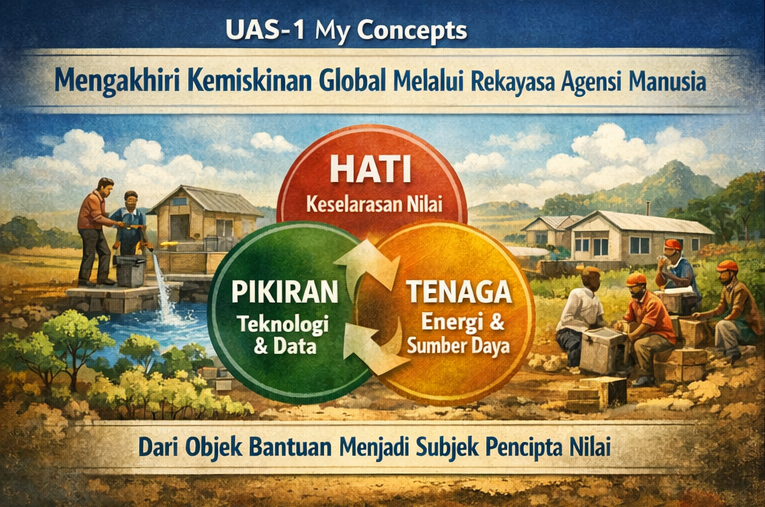
\includegraphics[width=9.5\linewidth,height=\textheight,keepaspectratio]{My_Concepts/../My_Concepts/1_My-Concepts.png}

}

\caption{My Concepts}

\end{figure}%

Konsep saya tentang pengentasan kemiskinan global tidak berangkat dari
pendekatan karitatif, melainkan dari rekayasa sistem yang memulihkan
agensi manusia. Kemiskinan ekstrem yang dialami sekitar 700 juta
penduduk dunia bukan sekadar kegagalan ekonomi, tetapi kegagalan sistem
global dalam menyelaraskan nilai, pengetahuan, dan kerja manusia.
Masalah utamanya adalah ketimpangan akses terhadap sistem penciptaan
nilai.

Saya memandang kemiskinan sebagai krisis koordinasi global. Individu
miskin tidak kekurangan potensi, mereka terputus dari sistem yang
memungkinkan potensi itu bernilai. Kemiskinan global bukan sekadar
masalah kelangkaan sumber daya, melainkan kegagalan sistemik dalam
menyelaraskan kecerdasan kolektif kita. Oleh karena itu, Mahakarya
Rekayasa untuk kemiskinan harus membangun ekosistem yang menyatukan
Hati, Pikiran, dan Tenaga dalam satu arsitektur pemberdayaan. Untuk
mewujudkan SDG 1 (Tanpa Kemiskinan) sebagai sebuah ``Mahakarya'', kita
harus menerapkan arsitektur Triune Intelligence (TISE) pada skala makro:

\begin{itemize}
\tightlist
\item
  \textbf{Hati (Homocordium - Axiological Intelligence):} Hati adalah
  kecerdasan nilai kolektif. Dalam konteks kemiskinan, ``Hati'' berarti
  pengakuan martabat manusia miskin sebagai aktor utama, bukan objek
  belas kasihan. Tanpa keselarasan nilai ini, kebijakan dan teknologi
  hanya menjadi instrumen dingin yang gagal menyentuh akar masalah.
  Komunikasi publik dan partisipasi komunitas menjadi mekanisme utama
  untuk menyelaraskan kecerdasan hati, sehingga solusi yang dirancang
  benar-benar menjawab kebutuhan riil di lapangan.
\end{itemize}

Ini adalah fondasi moral pengentasan kemiskinan. Kita harus mengubah
narasi dari ``memberi sedekah'' menjadi ``memulihkan martabat''.
Homocordium global harus bergetar pada frekuensi yang sama: bahwa
kemiskinan di Sub-Sahara Afrika adalah luka pada tubuh kemanusiaan
kolektif. Tanpa ``Hati'' yang terkalibrasi, bantuan kemanusiaan hanya
menjadi transaksi logistik tanpa empati yang mendalam.

\begin{itemize}
\tightlist
\item
  \textbf{Pikiran (Homodeus - Synergistic Practical Intelligence/PI-A):}
  Pikiran adalah kecerdasan rekayasa dan kecerdasan buatan. Di sinilah
  data kemiskinan, seperti ambang USD 2,15 per hari, diolah menjadi peta
  masalah yang presisi. AI berperan sebagai penguat daya pikir manusia.
  AI memetakan pola kerentanan, rantai pasok yang timpang, dan peluang
  ekonomi lokal. Namun, AI tidak mengambil keputusan moral. Manusia
  tetap menjadi pengarah utama yang menentukan prioritas dan tujuan
  sosial.
\end{itemize}

AI dan teknologi data bukanlah solusi ajaib, tetapi ``Juru Tulis
Cerdas'' bagi para pembuat kebijakan dan NGO. Kita menggunakan Homodeus
untuk memetakan kantong kemiskinan ekstrem secara real-time, memprediksi
krisis pangan sebelum terjadi, dan mengoptimalkan rantai pasok bantuan.
Namun, manusialah yang memegang kendali decision making untuk memastikan
algoritma tidak bias terhadap kelompok rentan.

\begin{itemize}
\tightlist
\item
  \textbf{Tenaga (Natural Intelligence - Human \& Environmental
  Energon):} Tenaga adalah energi kerja manusia dan sumber daya alam.
  Dalam kemiskinan ekstrem, tenaga manusia sering terbuang karena tidak
  terhubung ke sistem produktif. TISE mengelola tenaga ini melalui
  pendekatan PSKVE, sehingga waktu, keterampilan, dan sumber daya lokal
  dapat dikonversi menjadi produk, layanan, dan nilai ekonomi yang
  berkelanjutan. Tujuannya adalah memastikan setiap intervensi
  meningkatkan kapasitas jangka panjang, bukan sekadar konsumsi
  sementara.
\end{itemize}

700 juta orang yang hidup dalam kemiskinan bukanlah beban, melainkan
cadangan Human Energon yang belum teraktualisasi. Mahakarya ini terjadi
ketika kita menyuplai CORE Engine mereka dengan akses (kesehatan,
pendidikan), sehingga mereka dapat mengubah Time \& Effort mereka
menjadi nilai ekonomi (PSKVE) yang berkelanjutan, tanpa merusak
Environmental Energon.

Dengan demikian, Mahakarya Rekayasa untuk kemiskinan global bukanlah
program bantuan berskala besar, melainkan platform sistemik yang
menghubungkan jutaan komunitas miskin ke dalam jaringan ko-kreasi nilai
global. Platform ini memungkinkan setiap individu menjadi
Protagonis-Penulis atas kehidupannya sendiri, dengan dukungan sistem
yang adil, cerdas, dan berkelanjutan.

\bookmarksetup{startatroot}

\chapter{UAS-2 My Opinions ٩(ˊᗜˋ
)و}\label{uas-2-my-opinions-ux669ux2caux15dcux2cb-ux648}

\textbf{Opini Berpengaruh tentang Kemiskinan Global}

\begin{figure}[H]

{\centering 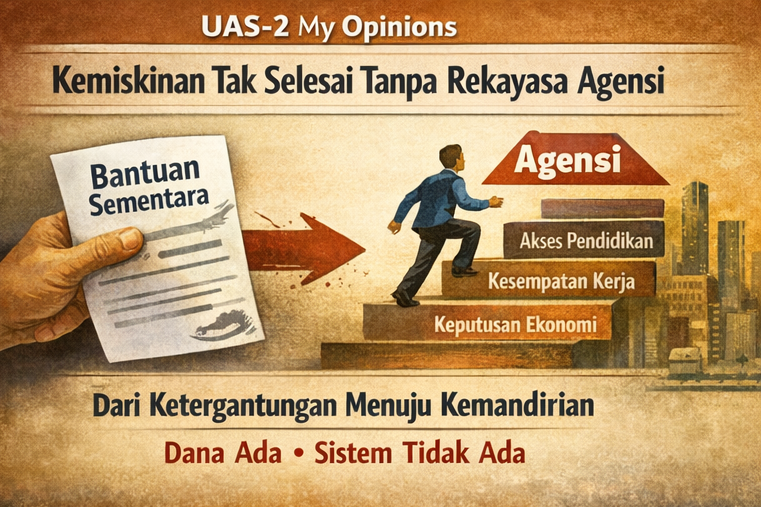
\includegraphics[width=9.5\linewidth,height=\textheight,keepaspectratio]{My_Opinions/../My_Opinions/2_My-Opinions.png}

}

\caption{My Opinions}

\end{figure}%

Pengentasan kemiskinan global selama puluhan tahun gagal karena fokus
pada distribusi, bukan pemberdayaan. Bantuan pangan, subsidi tunai, dan
hibah darurat memang menyelamatkan nyawa, tetapi tidak mengubah posisi
struktural masyarakat miskin dalam sistem ekonomi. Fakta bahwa
kemiskinan ekstrem meningkat kembali pasca pandemi COVID-19 menjadi
bukti nyata rapuhnya pendekatan lama.

Pendidikan, teknologi, dan kebijakan publik harus berhenti memposisikan
masyarakat miskin sebagai penerima. Mereka harus ditempatkan sebagai
pencipta nilai. Inilah pergeseran mental yang wajib dilakukan jika
Sustainable Development Goal 1 ingin tercapai secara nyata.

Opini saya tegas. Kemiskinan tidak dapat diselesaikan tanpa rekayasa
agensi. Selama orang miskin tidak memiliki kendali atas keputusan
ekonomi, pendidikan, dan kerja mereka, kemiskinan akan terus diwariskan.
Dunia saat ini tidak kekurangan dana, teknologi, atau pengetahuan. Dunia
kekurangan sistem yang menyatukan ketiganya dalam satu kerangka tujuan
kemanusiaan. Oleh karena itu, kta harus melakukan transformasi radikal
dalam cara kita memandang ``bantuan'' bagi kaum miskin, serupa dengan
pergeseran dari pembelajaran hafalan ke VALORAIZE Learning.

\begin{itemize}
\item
  \textbf{Kaum Miskin sebagai ``Protagonis-Penulis'':} Model bantuan
  konvensional sering kali menempatkan orang miskin sebagai objek pasif
  (seperti mahasiswa yang hanya menghafal jawaban). Kita harus mengubah
  mereka menjadi ``Protagonis-Penulis'' atas kisah hidup mereka sendiri.
  Mereka harus memiliki agensi untuk menentukan jalan keluar dari
  kemiskinan, bukan sekadar menerima paket bantuan standar.
\item
  \textbf{Ko-Kreasi Nilai di ``Pasar Kehidupan'':} Program pengentasan
  kemiskinan harus dirancang sebagai simulasi Knowledge Marketplace.
  Bantuan tidak diberikan cuma-cuma (yang menciptakan ketergantungan),
  tetapi dipertukarkan dengan ``Artefak Nilai'' yang mereka ciptakan.
\end{itemize}

\begin{quote}
\textbf{Contoh:} Petani miskin tidak hanya diberi uang, tetapi diberikan
modal untuk menghasilkan ``Peta Pertanian'' (rencana tanam) atau produk
lokal yang kemudian ``dibeli'' oleh pasar global atau pemerintah dengan
harga yang adil (mata uang fiat) atau akses layanan (mata uang
poin/sosial).
\end{quote}

\begin{itemize}
\tightlist
\item
  \textbf{Portofolio Kemandirian:} Keberhasilan program tidak diukur
  dari berapa dana yang disalurkan (ujian sesaat), tetapi dari
  Portofolio Kekayaan yang dibangun keluarga tersebut dari waktu ke
  waktu --- akumulasi aset, keterampilan, dan kesehatan yang membuktikan
  mereka telah lulus dari ambang batas USD 2,15 per hari.
\end{itemize}

\bookmarksetup{startatroot}

\chapter{UAS-3 My Innovations
◝(ᵔᗜᵔ)◜}\label{uas-3-my-innovations-ux1d54ux15dcux1d54}

\textbf{Inovasi TISE-Poverty: Teater Kerja Pengentasan Kemiskinan}

\begin{figure}[H]

{\centering 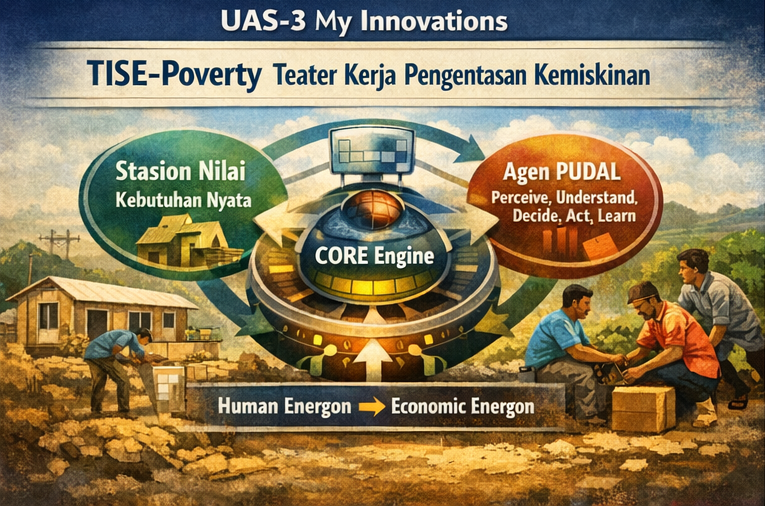
\includegraphics[width=9.5\linewidth,height=\textheight,keepaspectratio]{My_Innovations/../My_Innovations/3_My-Innovations.png}

}

\caption{My Innovations}

\end{figure}%

Inovasi utama saya adalah TISE-Poverty, sebuah arsitektur ``Teater
Kerja'' yang dirancang khusus untuk pengentasan kemiskinan ekstrem.
Teater kerja ini adalah ruang sosio-teknis tempat berbagai pemangku
kepentingan berkolaborasi secara terstruktur.

Di dalamnya terdapat Stasion Nilai, yaitu titik-titik di mana kebutuhan
nyata masyarakat didefinisikan. Contohnya akses air bersih, pekerjaan
lokal, atau pendidikan dasar. Untuk berpindah antar stasion, digunakan
Kendaraan berupa Agen PUDAL yang mampu memahami konteks lokal dan
mengorkestrasi solusi adaptif.

Agen PUDAL bekerja dengan siklus Perceive, Understand, Decide, Act, dan
Learn. Agen ini memanfaatkan data lokal, citra satelit, dan laporan
komunitas untuk merancang intervensi mikro. Contohnya penghubungan
petani kecil langsung ke pasar regional tanpa perantara, sehingga
pendapatan meningkat secara stabil.

Tenaga sistem ini disuplai oleh CORE Engine, yang mengonversi Human
Energon menjadi Economic Energon. Waktu dan keterampilan masyarakat
lokal diubah menjadi nilai ekonomi nyata melalui proyek berbasis
komunitas. Inovasi ini memastikan setiap solusi memiliki dampak jangka
panjang dan dapat direplikasi lintas wilayah.

\bookmarksetup{startatroot}

\chapter{UAS-4 My Knowledge ( ◡̀\_◡́)ᕤ}\label{uas-4-my-knowledge-_ux1564}

\textbf{Pengetahuan Baru tentang Kemiskinan sebagai Masalah Rekayasa
Sistem}

\begin{figure}[H]

{\centering 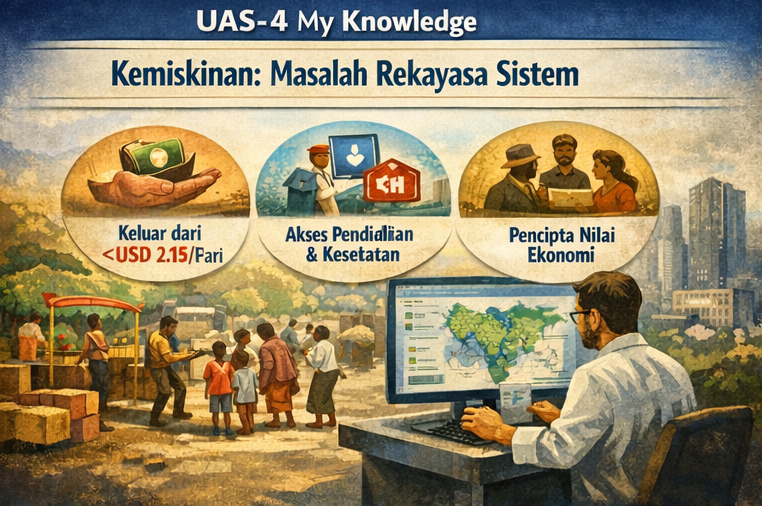
\includegraphics[width=9.5\linewidth,height=\textheight,keepaspectratio]{My_Knowledge/../My_Knowledge/4_My-Knowledge.png}

}

\caption{My Knowledge}

\end{figure}%

Mahakarya ini menghasilkan pengetahuan baru bahwa kemiskinan ekstrem
adalah kegagalan desain sistem sosial, bukan kegagalan individu.
Pengetahuan ini menuntut perubahan indikator keberhasilan. Keberhasilan
tidak lagi diukur dari jumlah bantuan yang disalurkan, tetapi dari
peningkatan agensi manusia.

Indikator utamanya adalah kemampuan individu keluar secara stabil dari
ambang USD 2,15 per hari, akses berkelanjutan terhadap pendidikan dan
kesehatan, serta keterlibatan aktif dalam sistem ekonomi lokal. Dengan
pendekatan ini, kemiskinan dipahami sebagai tantangan rekayasa yang
dapat dirancang, diuji, dan diperbaiki.

Mahakarya ini menegaskan satu hal. Jika rekayasa sistem mampu
menyelaraskan hati manusia, pikiran teknologi, dan tenaga kolektif, maka
kemiskinan ekstrem bukan takdir, melainkan masalah yang dapat
diselesaikan.

\bookmarksetup{startatroot}

\chapter{UAS-5 My Professional Reviews
ヾ(๑╹◡╹)ﾉ}\label{uas-5-my-professional-reviews-ux30feuxe51uxff89}

Rekap skor: Download file

\bookmarksetup{startatroot}

\chapter{Summary of Contents}\label{summary-of-contents}

\begin{itemize}
\item
  \hyperref[uts-1-all-about-me]{UTS-1 --- All About Me}: Perkenalan
  diri, latar belakang, hobi/minat, nilai yang dipegang, dan gagasan
  yang sedang dipikirkan. Nada personal, reflektif, dan hangat, dengan
  fokus pada proses bertumbuh dan eksplorasi di HMIF ITB (Media
  Intelligence).
\item
  \hyperref[uts-2-my-songs-for-you]{UTS-2 --- My Songs for You}: Karya
  lagu orisinal berjudul ``Stay a Little While'' terinspirasi dari Oasis
  --- lengkap dengan lirik, komposisi, dan embed Spotify untuk nuansa
  yang ingin disampaikan.
\item
  \hyperref[uts-3-my-stories-for-you-uxe51uxe51]{UTS-3 --- My Stories
  for You}: Cerita personal melewati masa sulit di awal kuliah,
  menemukan dukungan, dan bangkit. Menekankan makna kolaborasi, belajar,
  dan kehadiran orang terdekat sebagai kekuatan.
\item
  \hyperref[uts-4-my-shape-spiritual-gifts-heart-abilities-personality-experiences-ux3063]{UTS-4
  --- My SHAPE}: Peta diri terstruktur (Spiritual Gifts, Heart,
  Abilities, Personality, Experiences) beserta ``Piagam Diri'', prinsip
  kerja, serta narasi ringkas--panjang untuk merangkum misi, kekuatan,
  dan arah aksi.
\item
  \hyperref[uts-5-my-personal-reviews-uxe51ux3142ux648]{UTS-5 --- My
  Personal Reviews}: Metode self-assessment berbasis AI (ChatGPT) dengan
  rubrik UTS, hasil skor per kriteria, dan daftar prioritas perbaikan
  cepat. Menyertakan tautan unduhan ringkasan skor.
\item
  \hyperref[uas-1-my-concepts-ux3145]{UAS-1 --- My Concepts}: Konsep
  pengentasan kemiskinan sebagai rekayasa sistem yang memulihkan agensi
  manusia melalui TISE (Hati--Pikiran--Tenaga). Menempatkan kemiskinan
  sebagai krisis koordinasi global, bukan sekadar kekurangan sumber
  daya.
\item
  \hyperref[uas-2-my-opinions-ux669ux2caux15dcux2cb-ux648]{UAS-2 --- My
  Opinions}: Opini tegas tentang pergeseran dari distribusi bantuan
  menuju pemberdayaan. Menempatkan kaum miskin sebagai
  ``Protagonis-Penulis'' dan membangun portofolio kemandirian melalui
  ko-kreasi nilai.
\item
  \hyperref[uas-3-my-innovations-ux1d54ux15dcux1d54]{UAS-3 --- My
  Innovations}: Arsitektur inovasi ``TISE-Poverty: Teater Kerja'' dengan
  Stasion Nilai, Agen PUDAL (Perceive--Understand--Decide--Act--Learn),
  dan CORE Engine yang mengonversi Human Energon menjadi nilai ekonomi
  berkelanjutan.
\item
  \hyperref[uas-4-my-knowledge-_ux1564]{UAS-4 --- My Knowledge}:
  Pengetahuan baru yang menempatkan kemiskinan ekstrem sebagai kegagalan
  desain sistem sosial. Indikator keberhasilan bergeser ke peningkatan
  agensi dan keluarnya individu dari ambang USD 2,15/hari secara
  berkelanjutan.
\item
  \hyperref[uas-5-my-professional-reviews-ux30feuxe51uxff89]{UAS-5 ---
  My Professional Reviews}: Ringkasan dan tombol unduh skor profesional
  (XLSX) sebagai artefak evaluasi; melengkapi siklus UAS dengan bukti
  penilaian.
\item
  \href{references.qmd}{References}: Daftar pustaka yang digunakan dalam
  penyusunan karya.
\end{itemize}

\begin{quote}
Halaman ini merangkum isi utama dan menyediakan tautan cepat ke setiap
bagian.
\end{quote}

\bookmarksetup{startatroot}

\chapter*{References}\label{references}
\addcontentsline{toc}{chapter}{References}

\markboth{References}{References}

\phantomsection\label{refs}




\end{document}
